\documentclass{article}

\usepackage[danish]{babel}
\usepackage[utf8]{inputenc}
\usepackage{float}
\usepackage{fancyhdr}
\usepackage{amsmath}
\usepackage{color}
\usepackage{listings}
\usepackage{graphicx}
\usepackage{pdfpages}
\usepackage{booktabs}
%\usepackage{enumitem}
\lstset{language=R,basicstyle=\ttfamily\small}

\title{Statistik og dataanalyse \\ Tællende aktivitet 1}
\author{Peter Heilbo Ratgen - perat17@student.sdu.dk}
\date{\today}

\begin{document}
\maketitle
\newpage
\section{Databehandling}
Datafilen indeholder data om landes CO2-udledning per indbygger i metriske ton
per indbygger. Der er to kolonner i datafilen, "Country" og "CO2". Først gemmes
.xlsx-filen som en .csv fil. Denne data er dog ikke komplet, det indeholder også de
lande eller territorier der ikke har opgivet data. Det giver ikke mening at
betragte disse lande i statistikken, derfor fjernes disse fra datasættet. Dette
gøres ved at fjerne alle datapunkter der har ".." som værdi.
Også datapunkter der ikke er lande skal også fjernes fra datasættet, derfor fjernes
alle datapunkter hvor "income" indgår i navnet med kommandolinjeværktøjet
\texttt{sed}. Her er der fjernet 10 datapunkter. Derudover fjernes datapunktet
"world" også, siden det noget der kan regnes frem til. Til sidst i
databehandlingen skal \lstinline|,| ændres til \lstinline|.|, for at R
importerer data som den korrekte type.

Nu kan data indporteres til R med:
\begin{lstlisting}[language=R]
co2  <- read.csv("CO2.csv", sep = ";", row.names = NULL)
\end{lstlisting}
Her bruges \lstinline|sep = ";"| til at indikere at værdierne i .csv formatet
ikke er separeret med et komma, men med et semikolon.

\section{Grafiske illustrationer}

\subsection{Histogram}

\begin{figure}[H]
  \centering
  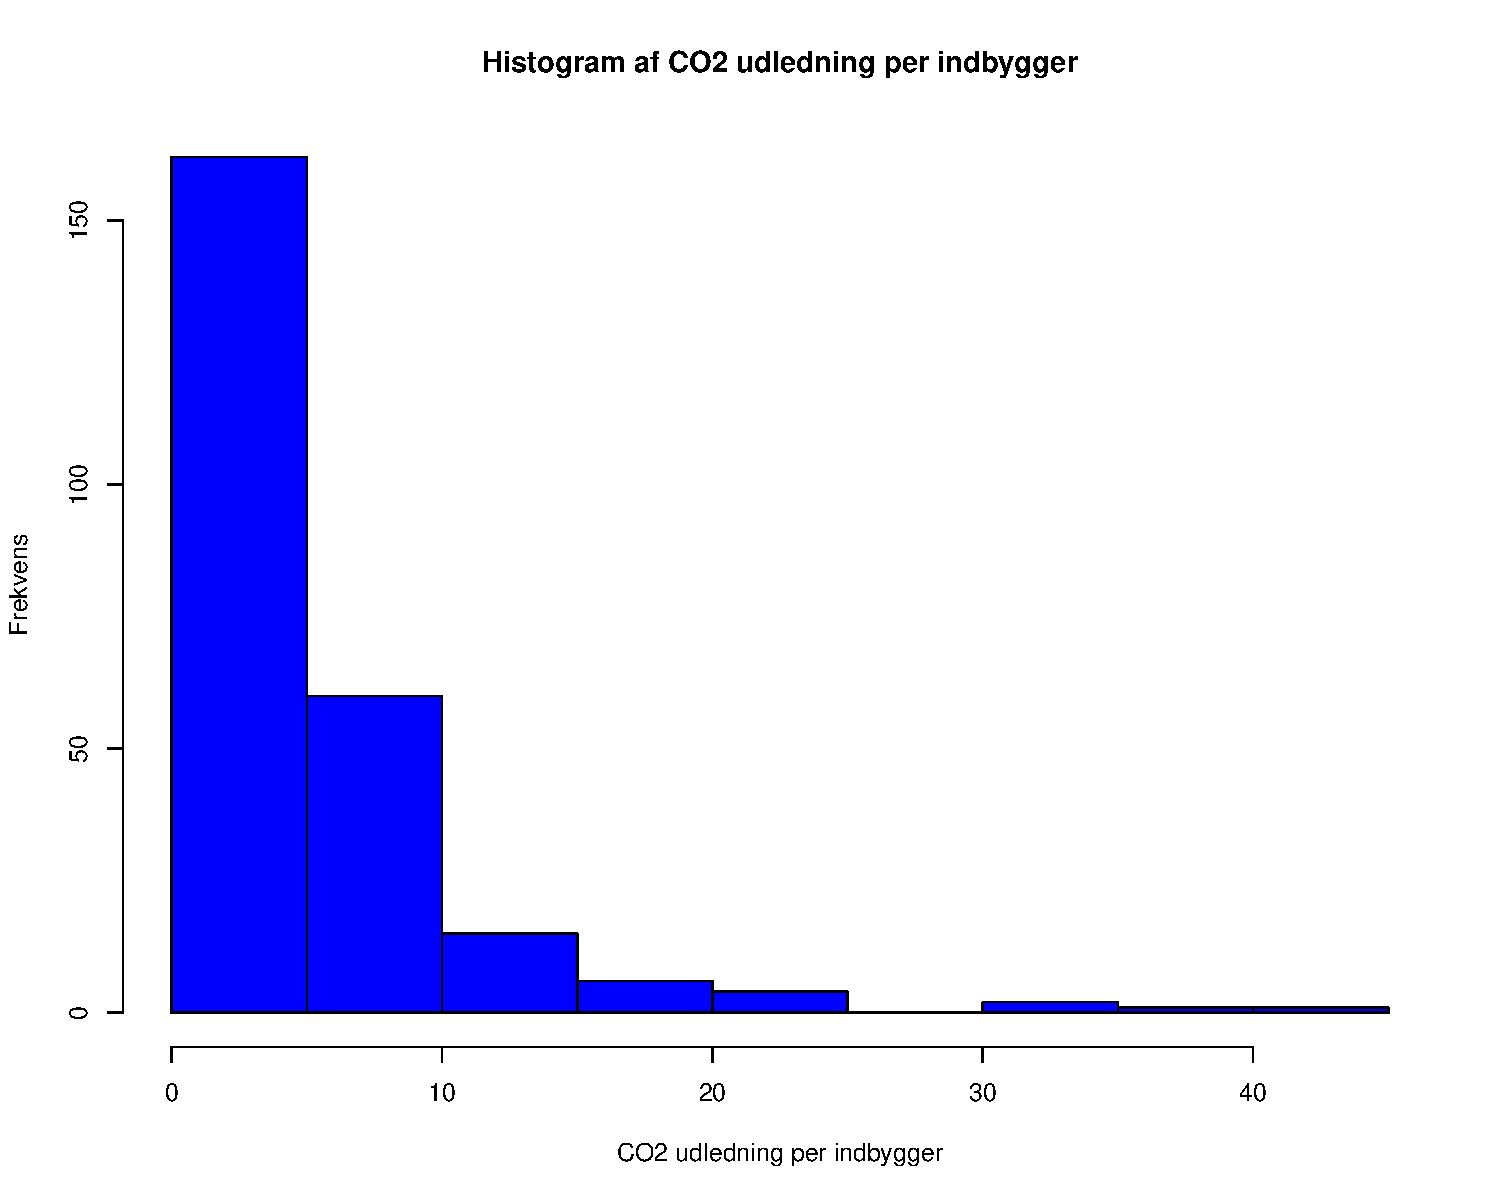
\includegraphics[width=0.8\textwidth]{co2plot.pdf}
\end{figure}

\subsection{Boxplot}

\begin{figure}[H]
  \centering
  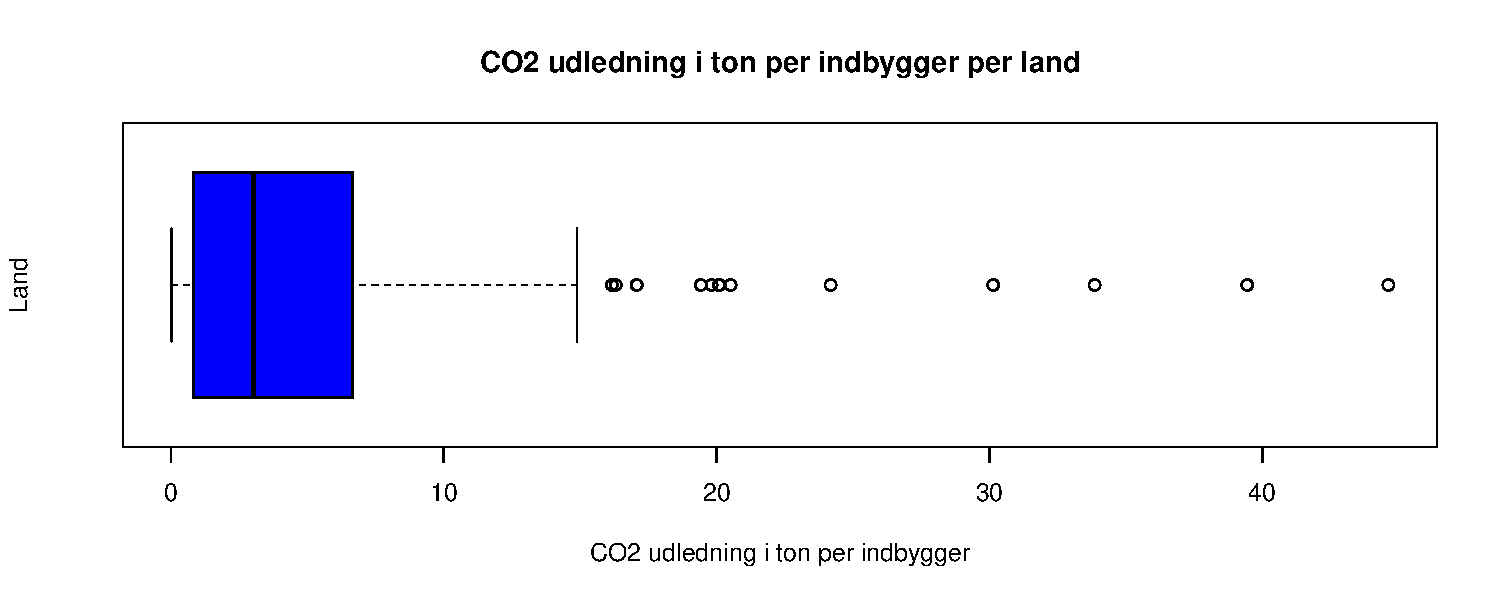
\includegraphics[width=0.9\textwidth]{co2boxplot.pdf}
\end{figure}

Boxplottet fortæller at langt de flest lande (75\%, eller dem inden for det 3.
kvartil) ikke udleder over 10 ton CO2 per indbygger. Det fortæller også at der
er nogle lande der udleder langt mere CO2 per indbygger, disse er de lande der
ligger uden for 1.5 gange den interkvatile afstand.

Danmark ligger indenfor det 3. kvartil med sine 6.51 ton CO2 udledt per
indbygger. Det vil også sige at Danmark ligger over medianen.

\section{Deskriptiv analyse}

\end{document}
